Das Bedrohungsmodel des theoretisch idealen Mix-Zone  Konzeptes \cite{Beresford2003} geht davon aus, dass der Benutzer eines Location Based Service diesen  nicht traut. Um aber diesen Service dennoch in Anspruch zu nehmen,  bedient er sich eines Middleware Systems  das als Proxy zwischen dem Nutzer und dem Location Based Service dient. Das Middleware System unterstützt ihn dabei seine Identität zu verstecken, indem der Nutzer  nur Service Callbacks über das Middleware System und in bestimmten dafür definierten Bereichen empfängt. Dafür meldet der Nutzer Interesse für ihn relevante Location Based Services bei der Middleware an und diese prüft periodisch den Ort des Nutzers und bestimmt, ob für den Nutzer ein relevantes Event ausgelöst worden ist und reicht ihm die Callbacks zu angemessenen Zeitpunkten weiter. Der Middleware Proxy benutzt Pseudonyme um die Identität des Nutzers vor dem Service zu verstecken.

Da Langzeit Pseudonyme  ermöglichen den Nutzer über spezifisches Verhalten, wie das Aufhalten an bestimmten Orten wie Zuhause oder auf Arbeit, die Identität zu ermitteln, schlägt \cite{Beresford2003} einen ständigen Pseudonymwechsel vor, auch wenn der Nutzer getrackt wird. Die Middleware versorgt den Nutzer regelmäßig mit neuen, unbenutzten pseudonymen für jede ortssensible Anwendung. Dieser Pseudonymwechsel findet innerhalb der sogenannten Mix-Zone statt. Allerdings können nur Location Bases Services genutzt werden, die Pseudonyme unterstützen.

Das Konzept der Mix Zone wird aus dem Konzept der Mix-Node aus dem Bereich der anonymen Kommunikationssystemen abgeleitet \cite{Chow2011}   Die Idee, die hinter dem Mix-Node liegt ist, dass er wartet bis er k Packtet mit gleicher Länge Empfangen hat und diese bevor er sie weiter leitet zufällig oder nach einer Metrik neu sortiert, so dass eine Unverknüpfbarkeit zwischen eingehenden und ausgehenden Paketen  entsteht.

\cite{Beresford2003} definiert eine Mix-Zone für eine Nutzergruppe als eine zusammenhängende Region mit maximaler Größe, in der keiner dieser Benutzer den Callback eines Location Based Service erhalten hat. Für diese Nutzergruppe können mehrere unterschiedliche Mix-Zones bestehen. Das Gegenstück zu einer Mix Zone ist die Application Zone, die als Gebiet, in der ein Nutzer einen Callback empfangen hat. Der Middleware Proxy kann die Mix-Zones im Voraus festlegen oder für jede Nutzergruppe einzeln als Gebiet festlegen in dem sich gerade kein Stück einer Application Zone befindet.

Weil standortbasierte Anwendungen in Mix-Zones keine ortsbezogenen Informationen erhalten, können sie Benutzer innerhalb der Mix Zone nicht unterscheiden. Und so kann eine Mix Zone die Unverknüpfbarkeit zwischen  eingehenden und ausgehenden Nutzern erreichen.

\begin{figure}[!h]
		\centering
		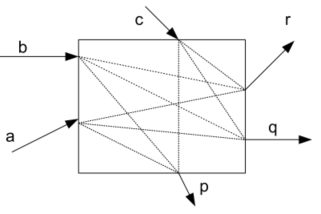
\includegraphics[width=0.5\textwidth]{Bilder/MixZone.PNG}
		\caption{Mix-Zone Model, Source: \protect\cite{Palanisamy2011}}
		\label{fig_Palanisamy2011}
	\end{figure}

\cite{Palanisamy2011} definiert das eine Mix-Zone Z k-anonymisierend  für eine Menge von Nutzern A ist wenn
\begin{enumerate}
\item Die Menge A mindestens k Elemente hat, $ |A| \geq k $.
\item Alle Nutzer in A müssen die Mix-Zone Z betreten haben, bevor ein Nutzer aus A die Mix-Zone Z verlässt.
\item Jeder Nutzer  der Menge A die Mix-Zone durch einen Eintrittspunkt $ e_{i} \in E $ betritt und diese durch einen Austrittspunkt $ o_{i} \in O $ verlässt und dabei eine zufällige Zeitspanne in der Zone verweilt.
\item Die Übergangswahrscheinlichkeit von jeden Eintrittspunkt zu jeden Austrittspunkt folgt einer Gleichverteilung.
\end{enumerate}

 \subsection{Mix-Zones über Straßennetze}
 
\cite{Palanisamy2011} beschreibt, dass die vorher betrachtete Definition der Mix-Zone davon ausgeht, dass sich die bewegenden Nutzer frei in einem euklidischen Raum bewegen ohne dass sie von räumlichen Beschränkungen betroffen sind. Im Normalfall in der Alltagswelt der mobilen Nutzer ist dies nicht so. So sind sie zum Beispiel durch Straßennetze und Fußgängerwege in ihrer freien Bewegung eingeschränkt. Die Mix-Zones für Straßennetze werde in der Regel einer Straßenkreuzung zugeordnet. Welche Straßenkreuzung als Standort einer Mix-Zone geeignet ist, hängt gewöhnlich von einer Reihe von Faktoren ab. Diese Faktoren beinhalten die Anzahl an Straßen, die an einer Kreuzung zusammen laufen, die Geschwindigkeit der mobilen Nutzer und Pfadbeschränkungen für mobile Nutzer, die sich innerhalb einer Mix-Zone aufhalten. Auch beeinflussen die ausgewählten Kreuzungen auf denen Mix-Zones errichtet werden sollen, auch die Anzahl der Eintritts- und Austrittspunkte der Mix-Zone, weil diese die eingehenden und ausgehenden Straßensegmente abbilden müssen und somit die Anzahl an Eintritts- und Austrittspunkten begrenzen. Auch liegen die Nutzer unter Beschränkungen durch das Straßennetz innerhalb einer Mix-Zone, so müssen sie sich an Geschwindigkeitsbegrenzungen halten und auch ihre freie Bewegung auf Grund von Straßen- und Gehsteigsführung eingeschnitten ist. Das resultiert dazu, dass Punkt (1), das zufällig Lange Aufhalten in einer Mix-Zone, und Punkt (2), die Gleichverteilung der Übergangswahrscheinlichkeiten  von Eintritts- und Austrittspunkten, in der Definition der k-Anonymität einer Mix-Zone verletzt werden. In den folgenden Absätzen wird erläutert, wie sich diese beiden Verletzungen nach \cite{Chow2011} der k-Anonymität auf den  Grad der Anonymität auswirken.

\begin{figure}[!h]
		\centering
		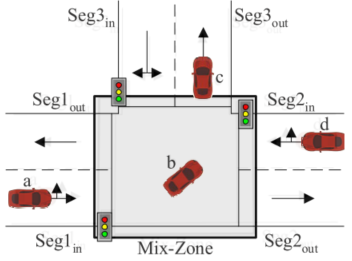
\includegraphics[width=0.4\textwidth]{Bilder/MixZoneNetwork.PNG}
		\caption{Mix-Zone eines Straßennetwerks, Source: \protect\cite{Chow2011}}
		\label{fig_MixSrasse}
	\end{figure}

1)	\textit{Mix-Zones ohne zufälliges Aufenthalten in ihr}: Sobald Nutzer eine unbestimmte Zeit in der Mix-Zone aufhalten, stellt eine zufällige Umordnung zwischen der Eintrittsreihenfolge und der Austrittsreihenfolge eine starke Unverknüpfbarkeit zwischen alten und neuen Pseudonymen sicher. Zum Beispiel, wenn alle Nutzer eine konstante Zeit in einer Mix-Zone verbringen, würde das System dem einfachen First-In-First-Out Prinzip entsprechen. Und somit kann dem ersten verlassenden Pseudonym das entsprechende erste eintretende Pseudonym zugeordnet werde und so weiter.

2)	\textit{Mix-Zones ohne gleichverteilte Übergangswahrscheinlichkeiten}: Sobald die Regel gelockert wird, dass die Übergangswahrscheinlichkeit zwischen Eintritts- und Austrittspunkt gleichverteilt sind wie in der theoretischen Mix-Zone, können einige Übergange zwischen Ein- und Austrittspunkten wahrscheinlicher werden als andere. Ein Angreifer könnte dieses Wissen nutzen, um  Verknüpfungen zwischen neuen und alten Pseudonymen zu folgern. Beispielhaft könnte ein Angreifer in einen solchen Szenario Übergänge, die weniger wahrscheinlich sind, aus seiner Abbildung der Pseudonyme entsprechend dieser Übergänge eliminieren und somit das Inferieren der Pseudonymverknüpfungen verbessern.

Aus diesen beiden Schwächen leitet \cite{Palanisamy2015} die drei Arten von Attacken auf Mix-Zones über Straßennetzwerken ab: (1) Timing Attacks, (2) Transaction Attacks und (3) Combined  Timing and Transition Attacks.

1)	\textit{Timing Attack}: Bei einer Timing Attack beobachtet der Angreifer die Eintritts- $t_{in}(i)$ und die Austrittszeit $t_{out}(i)$ für jeden Nutzer der die Mix-Zone durchquert. Sobald der Angreifer erkennt das ein Nutzer i' die Mix-Zone verlässt, versucht er i' auf einen Nutzer aus dem Anonymitätsmenge Ai ab zu bilden. Der Angreifer weißt der Wahrscheinlichkeit $p_{i'\rightarrow j}$ einen Wert zu, so dass dieser der Wahrscheinlichkeit i' auf j abzubilden entspricht, wobei $j \in A$. Die Abbildungswahrscheinlichkeiten werden berechnet durch Inference basierend auf den Wahrscheinlichkeiten von den übriggebliebenen Nutzer, das diese zum Austrittszeitpunkt $t_{out}(i')$ die Mix-Zone verlassen.  Nachdem die Abbildungswahrscheinlichkeiten berechnet worden sind, kann der Angreifer die Schiefe in der Abbildungswahrscheinlichkeitsverteilung nutzen um Abbildungen mit geringer Wahrscheinlichkeit  unter Abwägung zu entfernen und so die Anzahl der Nutzer aus A, die in Betracht kommen, einzugrenzen durch die Berücksichtigung von hoch wahrscheinlichen  Abbildungen.

2)	\textit{Transition Attack}: Bei einer Transition Attack schätzt der Angreifer die Übergangswahrscheinlichkeit für jede Abbiegemöglichkeit auf Grundlage vorheriger Beobachtungen. Beim Erkennen, dass ein Nutzer i' die Mix-Zone verlässt, weißt der Angreifer der Abbildungswahrscheinlichkeit $p_{i'\rightarrow j}$  für jedes $j \in A$ auf Grundlage der Bedingten Übergangswahrscheinlichkeiten T(iseg(i), oseg(i')) und T(iseg(j), oseg(i')).  T(iseg(j), oseg(i')) ist dabei die Notation der Bedingten Wahrscheinlichkeit eines Nutzers i' der durch Straßensegment iseg(j) die Mix-Zone betreten hat unter der Bedingung diese über das Straßensegment oseg(i') verlassen hat. Die Abbildungwahrscheinlichkeiten  $p_{i'\rightarrow i}$ und $p_{i'\rightarrow j}$ unter einer Transition Attack sind daher durch \\
$p_{i'\rightarrow i} = \dfrac{T(iseg(i), oseg(i'))}{T(iseg(i), oseg(i')) + T(iseg(j), oseg(i'))} $\\
 und \\
  $p_{i'\rightarrow j} = \dfrac{T(iseg(j), oseg(i'))}{T(iseg(i), oseg(i')) + T(iseg(j), oseg(i'))} $ \\ gegeben.
  
 3)	\textit{Combined  Timing and Transition Attack}: Bei dieser Art von Angriff ist der Angreifer sowohl wissend über die Ein- und Austrittszeiten der Nutzer als auch den Übergangswahrscheinlichkeiten an Kreuzungen der gegebenen Mix-Zone des Straßennetzwerks. Der Angreifer kann  daher die Abbildungswahrscheinlichkeit $p_{i'\rightarrow j}$ für jedes $j \in A$ basierend auf den Wahrscheinlichkeiten des Nutzers j zum Zeitpunkt $t_{out}(i')$ die Mix-Zone verlässt und den Bedingten Übergangswahrscheinlichkeiten $T(iseg(j), oseg(i'))$ schätzen. 
 
 \begin{figure}[!h]
 	\centering
 	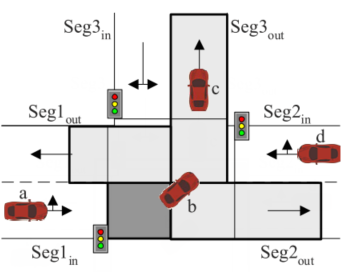
\includegraphics[width=0.4\textwidth]{Bilder/nonrectangularMix.PNG}
 	\caption{Non-Rectangular Mix-Zone, Source: \protect\cite{Chow2011}}
 	\label{fig_MixSrasseNon}
 \end{figure}
 
 Da eine einfache rechteckige Mix-Zone um eine Straßenkreuzung diesen Attacken nicht ausreichend stand hält, haben [Palanisamy2015, Palanisamy2011] die Time Window Bounded Non-Rectangular Mix-Zones entworfen. Dieser Typ von Mix-Zone besteht aus mehreren rechteckigen Teilstücken.  Diese beginnen von der Mitte der Kreuzung und liegen nur auf den ausgehenden Straßensegmenten der Kreuzung  (siehe Abbildung \ref{fig_MixSrasseNon}). Dieser Ansatz wird im Folgenden als Non-Rectangular Ansatz bezeichnet. Dieser Ansatz schützt besser vor Timing Attacks, die auf der Heterogenität der  Geschwindigkeitsverteilung auf den Straßensegmenten basieren. Es wird angenommen, das sie Anonymitätsmenge für jeden Nutzer i alle Nutzer beinhaltet, die die Mix-Zone in einem Zeitfenster mit dem Intervall $| t_{in}(i)-\tau_{1}|$ bis $|t_{in}(i)+\tau_{2}|$ betreten haben. $t_{in}(i)$ ist der Eintrittszeitpunkt des Nutzers i und ta1 und ta2 werden als so kleine Werte gewählt, dass das Zeitfenster sicherstellt, dass die Anonymitätsmenge von i nur Nutzer ähnlich naher Ankunftszeit beinhaltet. Die Länge der Mix-zone auf den ausgehenden Straßensegmenten  wird basierend auf der Geschwindigkeit des Straßensegments, der Größe des Zeitfensters und dem benötigten Anonymitätsgrad bestimmt.     